\subsection{Ridge regression}

Now we applied the ridge regression to perform variable selection. In \Fig~\ref{fig:RidgeCoefVsLambda} is shown the coefficients' behavior as $\lambda$ increases. 

It is possible to observe that for enough large values of $\lambda$, around $10^2$, all the coefficients tend to become close to zero. However, they are never exactly zero.

To select the optimal value of the penalization factor $\lambda$ we employed \textit{k}-fold cross-validation with $\textit{k}=10$. In \Fig~\ref{fig:RidgeCvPlot} it is possible to observe the trend of the cross-validated mean square error (MSE) when $\lambda$ increases. The optimal value was found to be $\lambda_{opt} = 0.0268$.

\begin{figure}[h]
	\centering
	\begin{subfigure}{.5\textwidth}
		\centering
		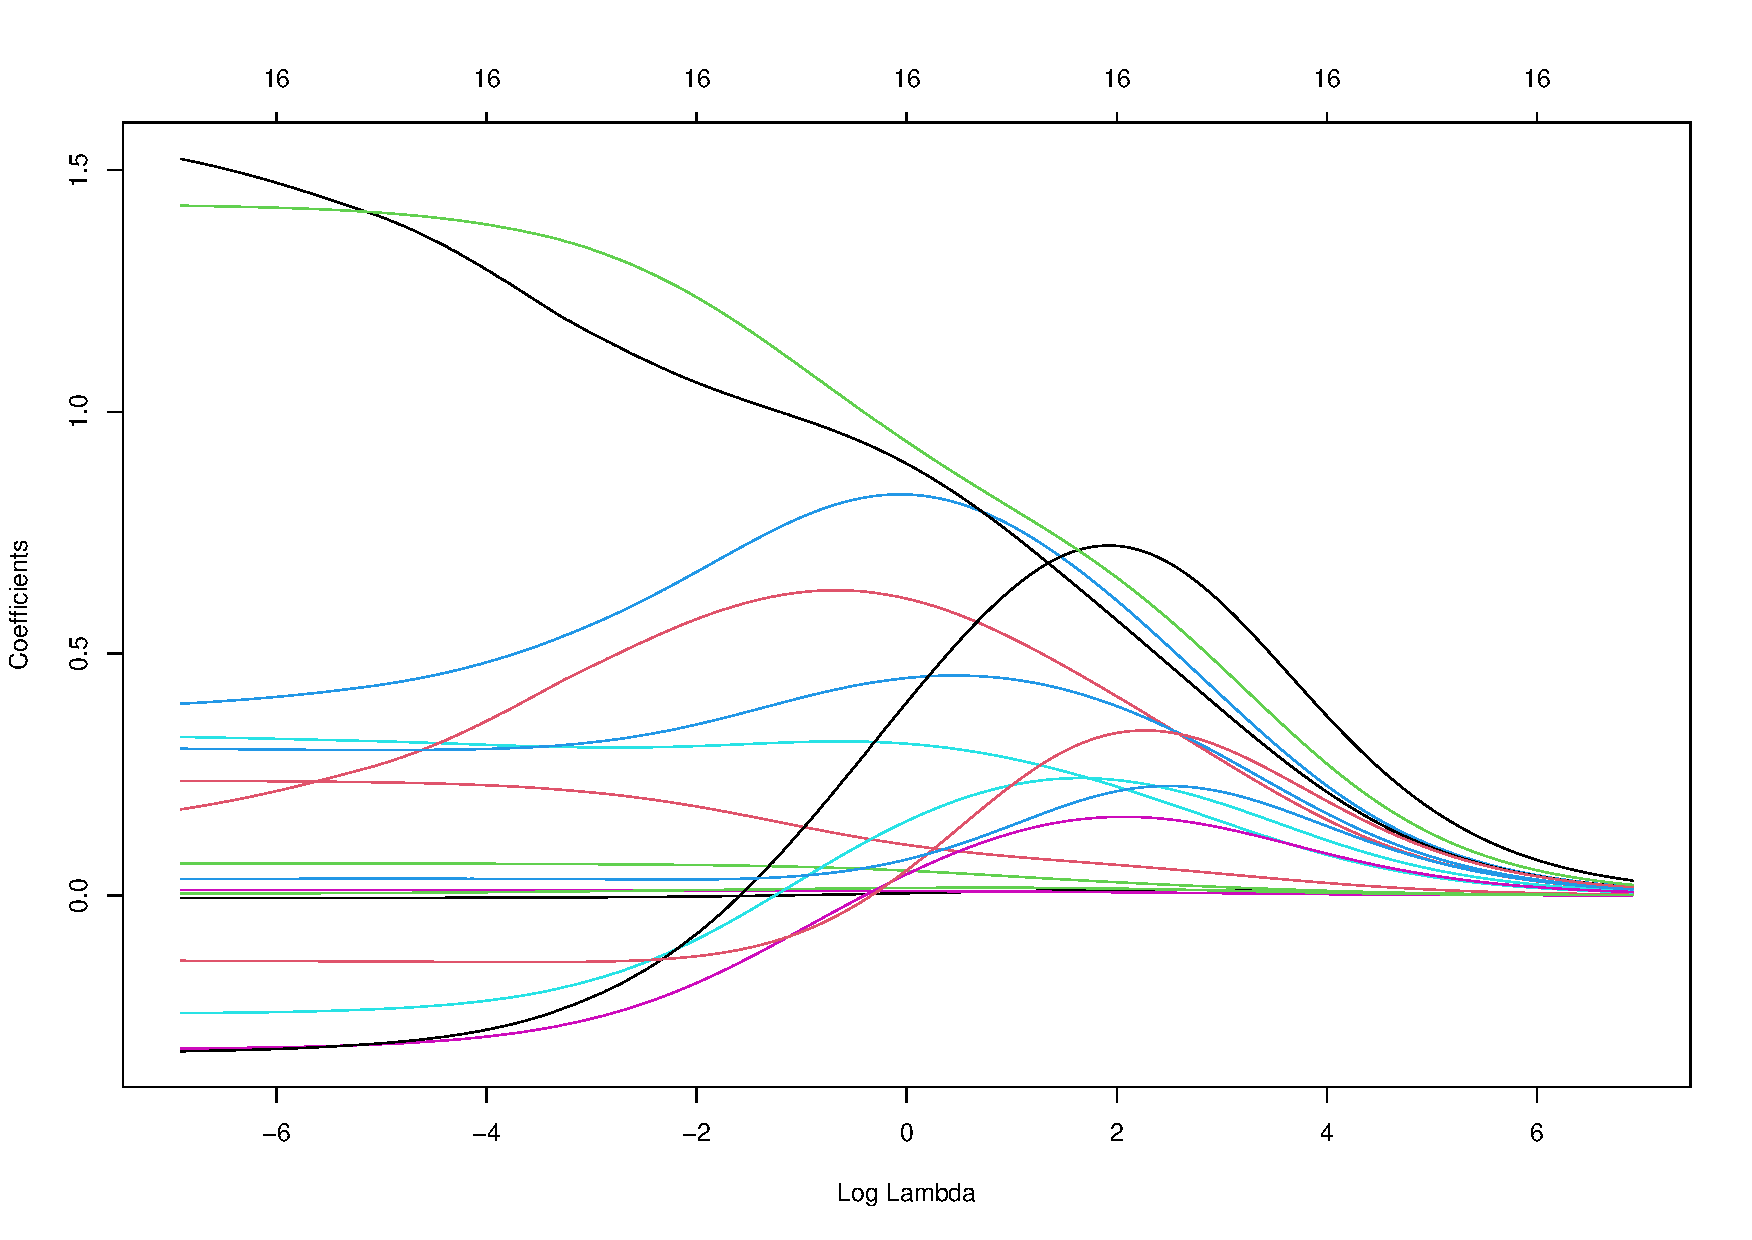
\includegraphics[width=0.7\linewidth]{ImageFiles/Regression/Ridge/RidgeCoefVsLambda.pdf}
		\caption{}
		\label{fig:RidgeCoefVsLambda}
	\end{subfigure}%
	\begin{subfigure}{.5\textwidth}
		\centering
		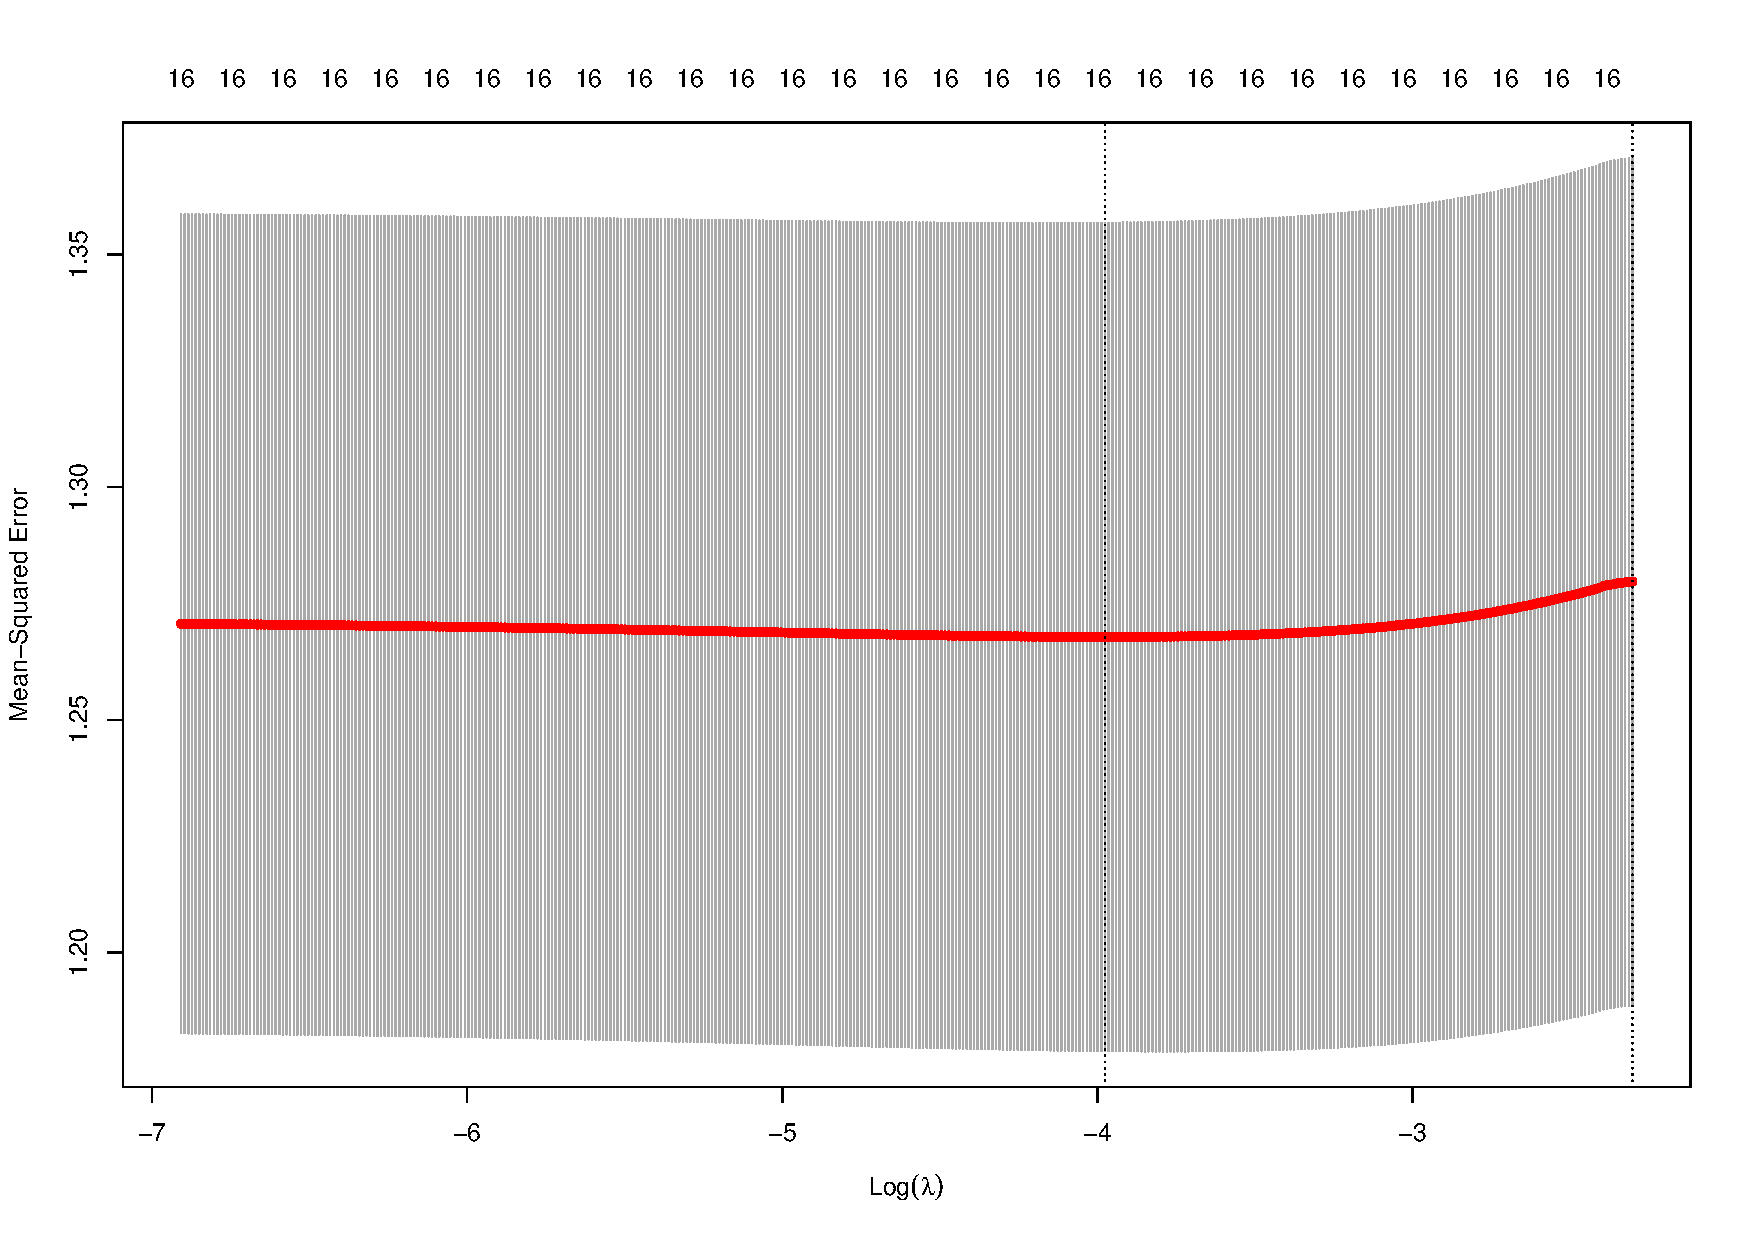
\includegraphics[width=0.7\linewidth]{ImageFiles/Regression/Ridge/RidgeCvPlot.pdf}
		\caption{}
		\label{fig:RidgeCvPlot}
	\end{subfigure}
	\caption{Application of ridge regression with different values of $\lambda$. (a) Coefficients as a function of $\lambda$. (b) Cross-validation MSE as a function of $\lambda$.}
	\label{fig:FinalFSSM}
\end{figure}

We fit the final model using $\lambda_{opt}$. The resulting coefficients are displayed in \Tab~\ref{table:FinalRidgeCoef}. For this model the computed MSE is 1.2577.

